\documentclass[
%*********************************************
%* Paper type (letterpaper)                  *
%*********************************************
    a4paper,
%   letterpaper,
%   a5paper,
%   b5paper,
%   executivepaper,
%   legalpaper,
%
%*********************************************
%* Font size (10pt)                          *
%*********************************************
%   10pt,
    11pt,
%   12pt,
%
%*********************************************
%* Paging (document dependent)               *
%*********************************************
    oneside,
%   twoside,
%
%*********************************************
%* Equation alignment (center)               *
%*********************************************
%   fleqn,                  %placerer fomlerne i venstre siden istedet for centreret.
%   leqno,                  %Placerer formelnummereringen på venstre side (istedet for højre)
%
%*********************************************
%* Chapter positioning (document dependent)  *
%*********************************************
    openany,                %openany starter chapters på næstkommende side.
%   openright,
%
%*********************************************
%* Language (none)                           *
%*********************************************
%    english]
   danish]
%
%*********************************************
%* Document type (none)                      *
%*********************************************
%   {book}
    {article}
%   {slides}
%   {report}


%*********************************************
%* Userpackages                              *
%*********************************************
\usepackage[danish]{babel}
%\usepackage{t1enc}          %Bruges til sprog oa.
\usepackage[latin1]{inputenc}
\usepackage{amsfonts}
\usepackage{mathrsfs}
%\usepackage[xdvi]{epsfig}
%\usepackage{ifthen}
%\usepackage{latexsym}
%\usepackage{theorem}
\usepackage{graphicx}       %Used when including .eps (graphics) files
%\usepackage{varioref}
%\usepackage{epic}
%\usepackage{eepic}
%\usepackage{rotfloat}
%\usepackage{multicol}
%\usepackage{wrapfig}
%\usepackage{syntonly}          %Use this to check for proper syntax, makes output file.
%\syntaxonly                %Use this to check for proper syntax, makes NO output file.
\usepackage{verbatim}          %Used when to include an unformatted ASCII file
%\usepackage{fancyhdr}
%\usepackage{layout}
%\usepackage{float}
%\usepackage{makeidx}          %Used when making an index in the document
\usepackage{calc}              %Used if you wanna use cm, mm, ex etc. instead of pt

%%
%% For code syntax highliting
%%
%\usepackage{color}
%\usepackage{alltt}

\pagestyle
%*********************************************
%* Header / footer configuration (none)      *
%*********************************************
    {plain}                 %Writes page number in footer, header is empty.
%   {headings}
%   {empty}                 %Makes no header or footer
%   {myheadings}
%   {fancy}



%*********************************************
%* Extra pagelayout    (se s. 110)           *
%*********************************************
%\hoffset   =   -0.5cm %Venstremargin
%\voffset   =   0pt
%\evensidemargin=   0pt
%\oddsidemargin =   0pt %Ekstra venstremargin til dobbeltsider
%\topmargin =   -2cm
%\headheight    =   0pt
%\headsep   =   0pt
%\textheight = 690pt
%\textwidth =   480pt
%\marginparsep  =   0pt
%\marginparwidth=   0pt
%\footskip  =   0pt
%\marginparpush =   0pt
%\paperwidth    =   597pt
%\paperheight   =   845pt

%\makeindex

%\parskip   =   1ex
%\parindent =   0em
%\baselineskip  =   2ex

%\underlineheadings

\title{M�ling af NXT-h�jttaler
\\
\vspace{2cm}
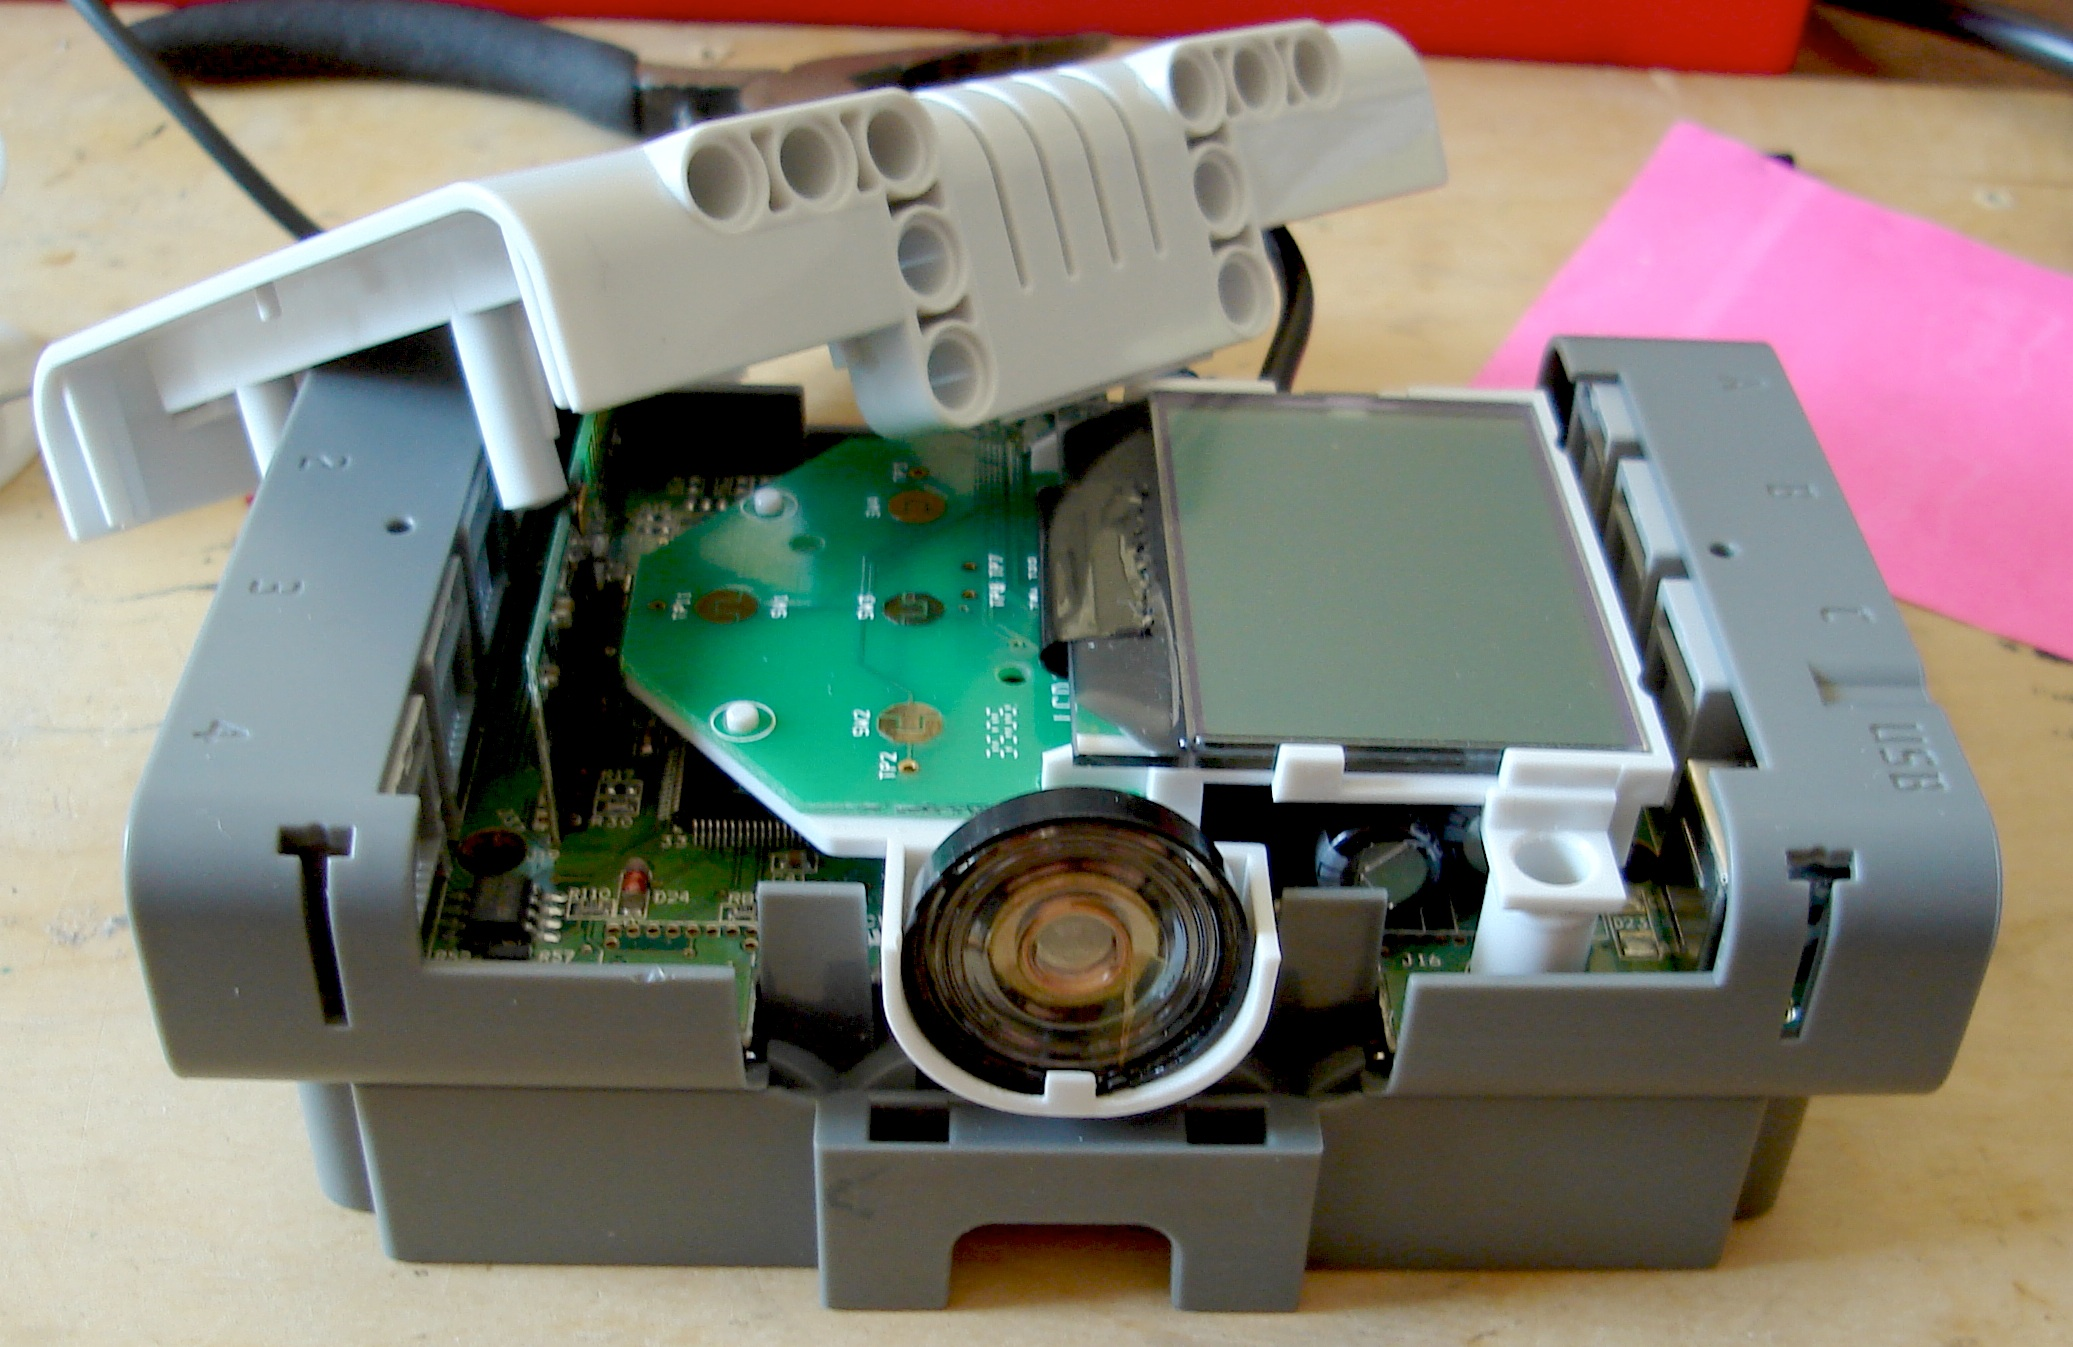
\includegraphics[width=10cm]{nxt-open-front.jpg}
}
%
\author{Mikkel Gravgaard - 20043246\\Bent Bisballe Nyeng - 20001467}

\markboth{}{}
%*********************************************
%*                start of                   *
%*              -=DOCUMENT=-                 *
%*********************************************
\begin{document}
\maketitle
\tableofcontents 
Vi ønsker i denne øvelse at implementere billedkomprimering ved hjælp af de teknikker som benyttes i JPEG, nemlig kvantisering af en frekvensmatrice samt Huffman-kodning.

Vi ønsker at konstruere vores program således at det er muligt for brugeren at eksperimentere med forskellige kvantiseringsindstillinger.



\section{M�leopstillinger}
P� hardware-siden har vi benyttet en b�rbar Mac tilkoblet et Alesis
IO|14 lydkort. Vi har foretaget m�lingerne ved hj�lp af softwaren
FuzzMeasure 2\footnote{\texttt{http://www.supermegaultragroovy.com/products/FuzzMeasure/}}.

Ved hj�lp af FuzzMeasure har vi sendt et sinus-sweep (1000 ms
varighed, g�ende fra 100 Hz til 20 kHz) igennem NXT-h�jttaleren og
optaget det igen. FuzzMeasure beregner impulssvaret ved at affolde
sinus-sweepet fra det optagede signal. Vi har optaget signalet ved
48 kHz, s�ledes at vi b�de har taget Nyquist samt high-cut filteret
p� lydkortets A/D-converter i betragtning.

Til vores m�linger har vi benyttet en Behringer ECM8000 m�lemikrofon,
som har en nogelunde line�r frekvensgang indenfor det frekvensomr�de
vi er interresserede i at unders�ge, dvs. 100Hz til 20kHz. Mikrofonens
frekvens karakteristik kan ses p� figur \ref{ecm8000}.

\begin{figure}[h!]
\begin{center}
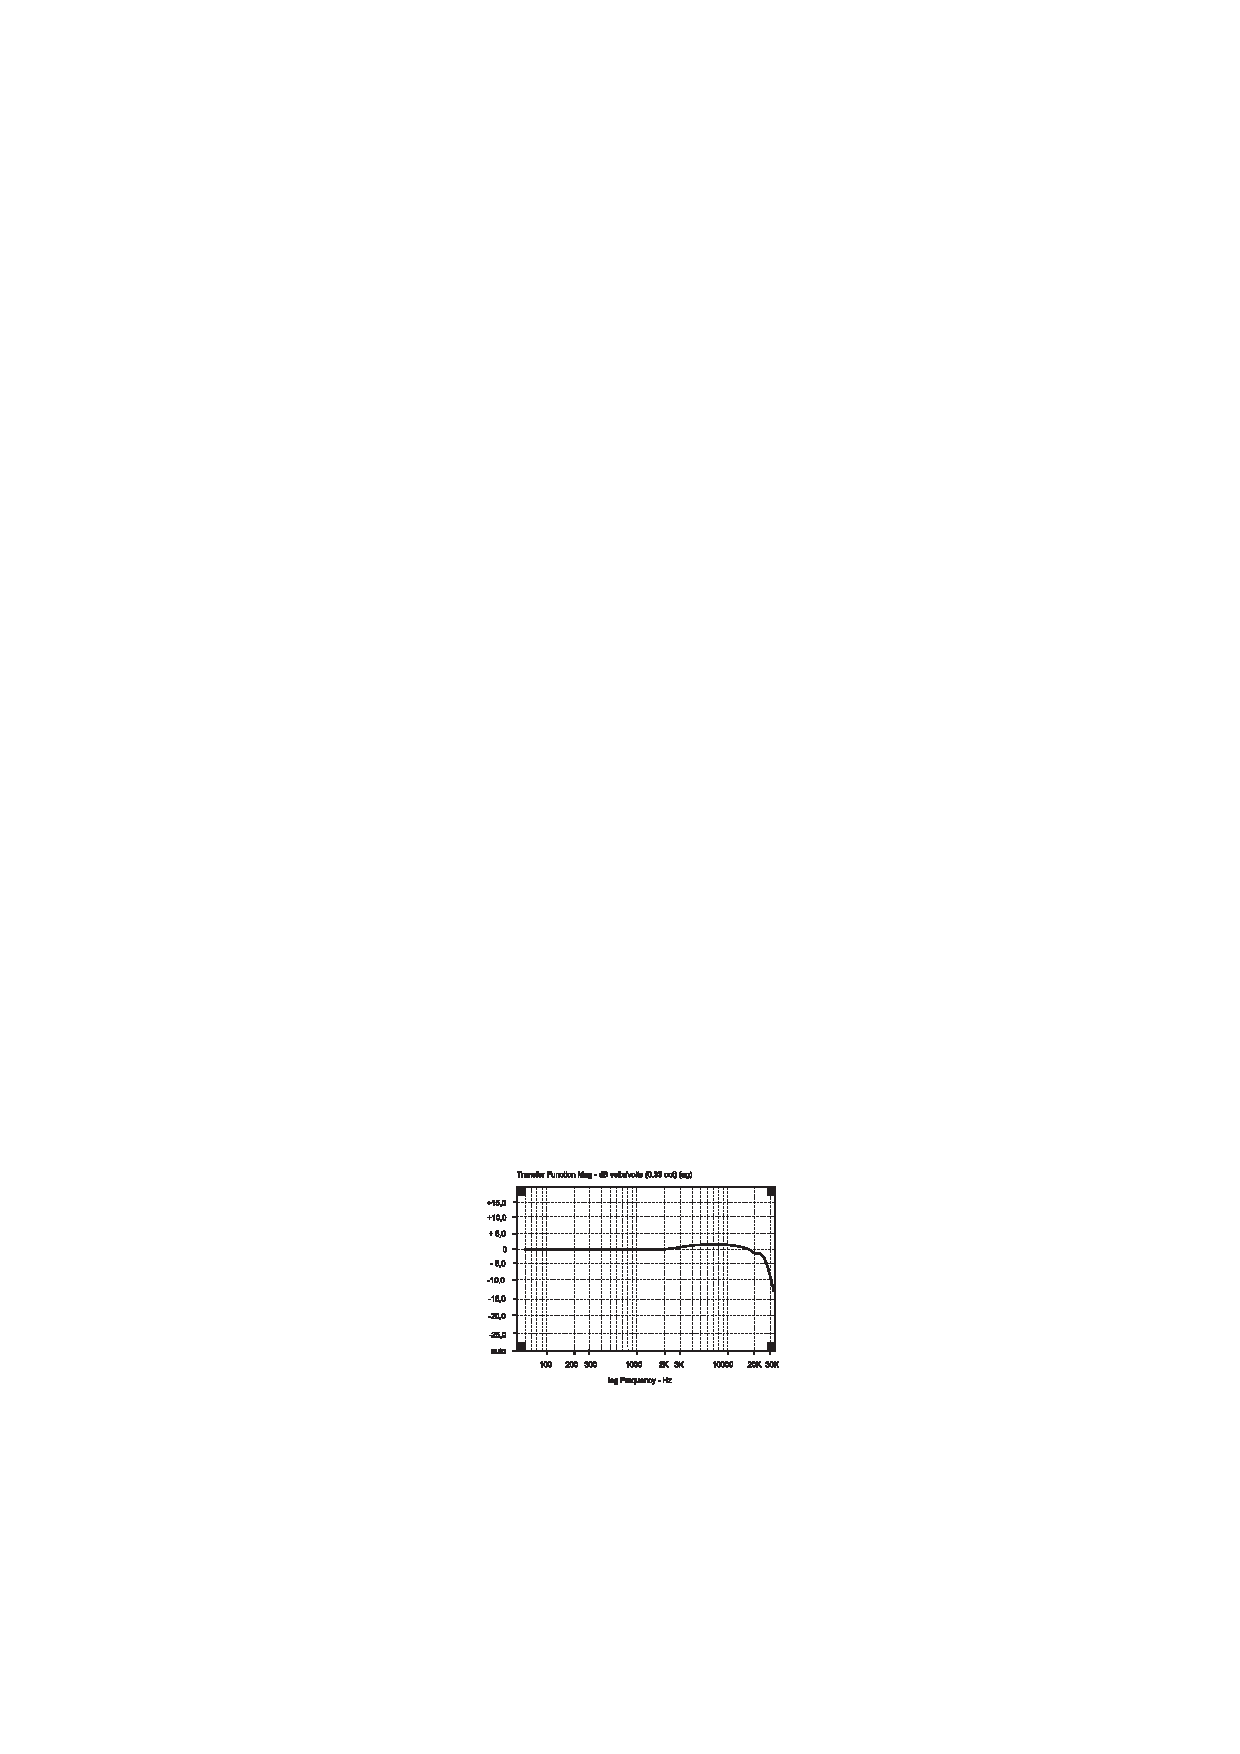
\includegraphics[width=12cm]{ecm8000_freqres.pdf}
\end{center}
\caption{Frekvensgangen p� Behringer ECM8000 mikrofonen}
\label{ecm8000}
\end{figure}

Vi har m�lt i 10 graders intervaller op til 40 grader fra on axis og i
alle retninger. I alt 81 m�linger.\\
Det giver anledning til det grid over m�lingerne, som kan ses p� figur
\ref{angles}.
\begin{figure}[h!]
\begin{center}
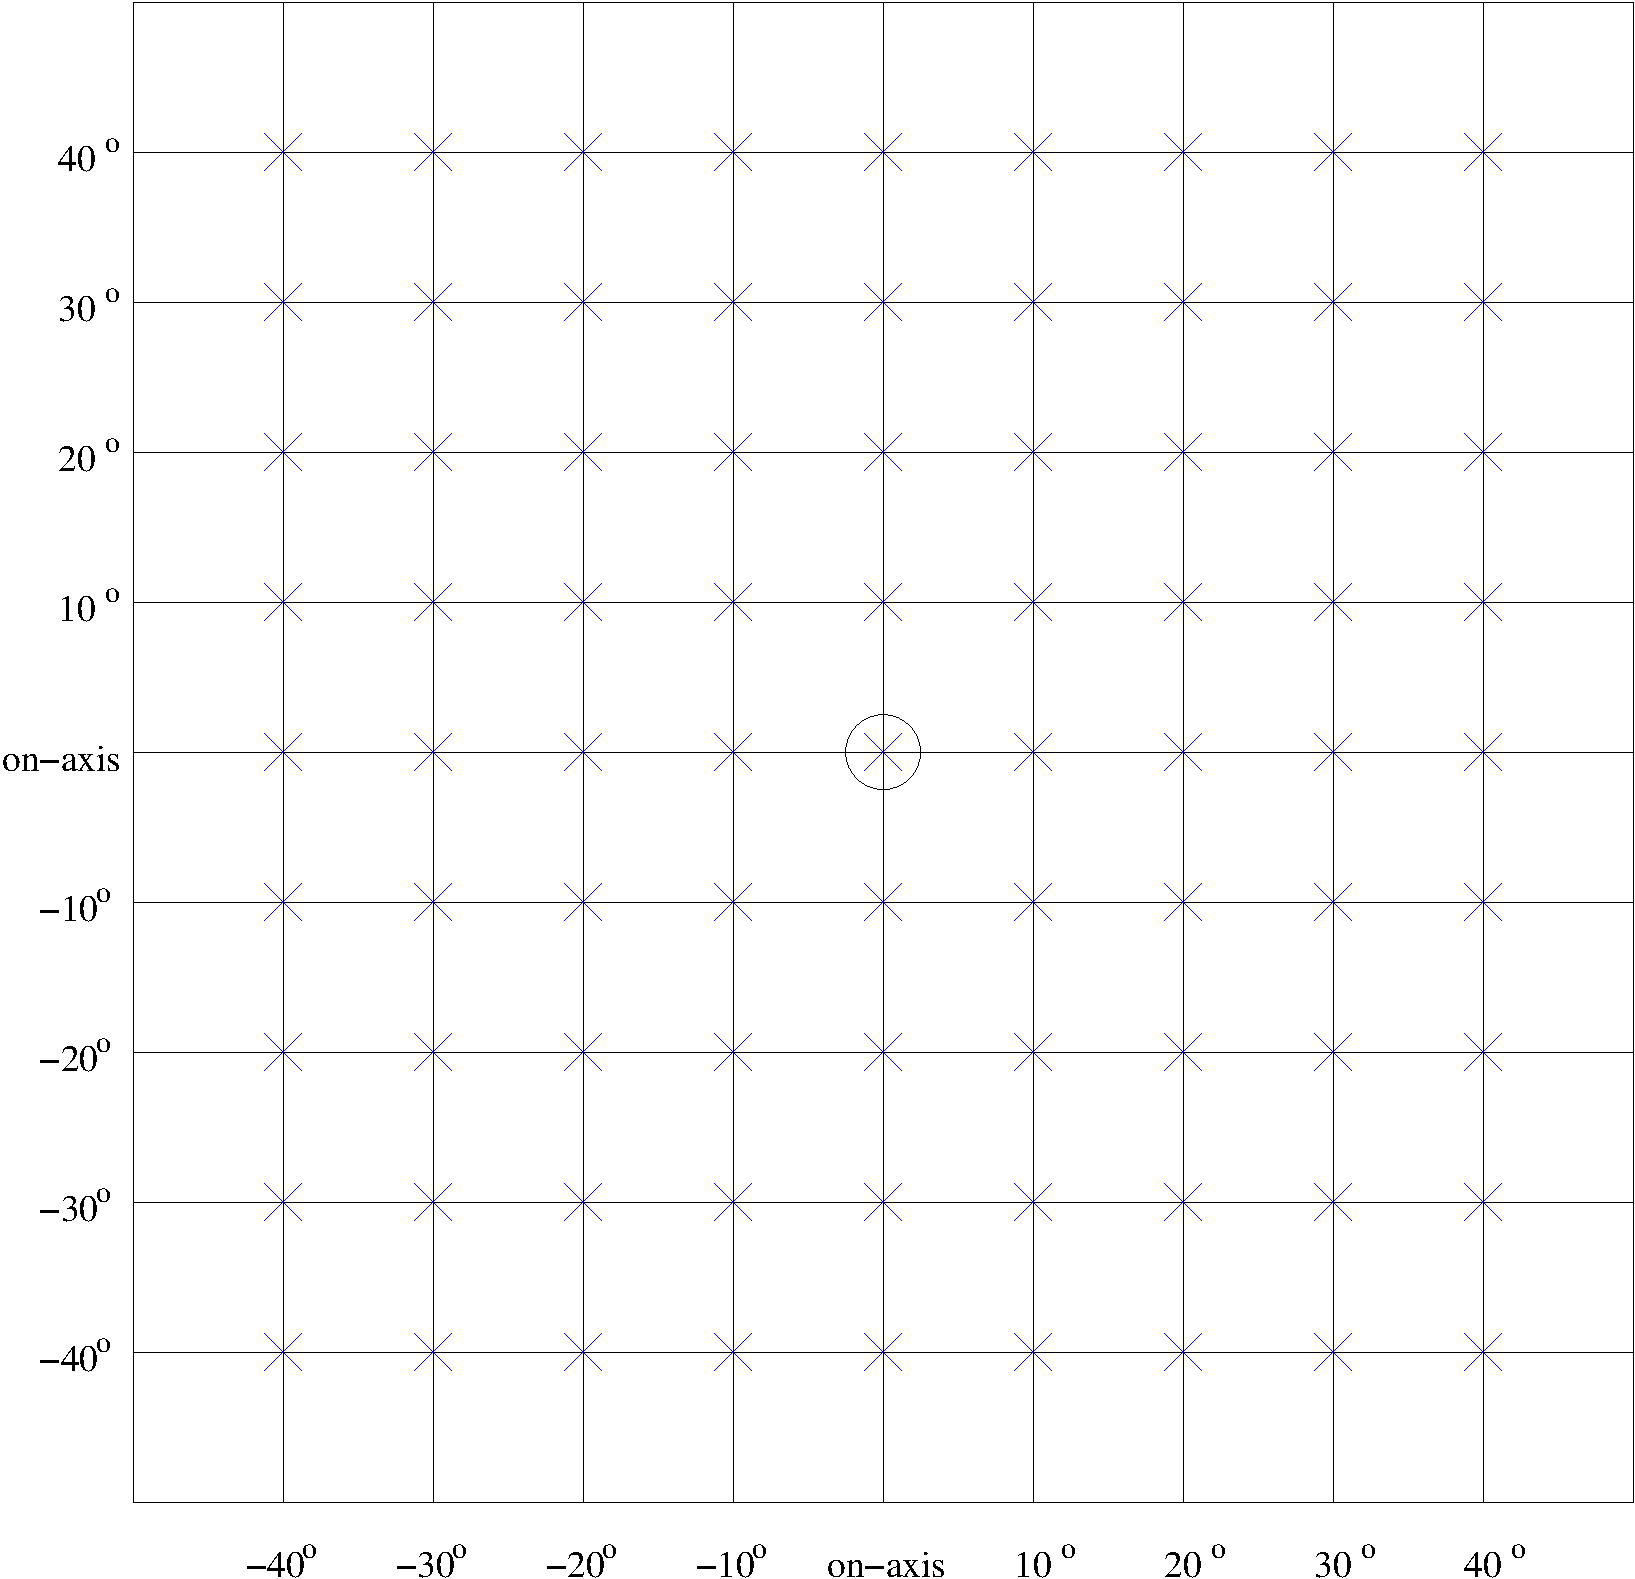
\includegraphics[width=8cm]{angles.pdf}
\end{center}
\caption{Illustration af m�lepunkterne.}
\label{angles}
\end{figure}

For at kunne m�le direkte p� h�jttaleren har vi skildt NXT'en ad og
loddet et kabel direkte p� polerne.\\
For at kunne lave m�linger af h�jttalerens kabinet (NXT'ens
plastikkasse) har endvidere indf�rt h�jttaleren p� sin oprindelige
plads i kabinettet med tilh�rende gennemf�ring af kablet.\\
Billeder af den afkoblede h�jttaler med lodninger kan ses p� figur \ref{lodning} 
\begin{figure}[h!]
\begin{center}
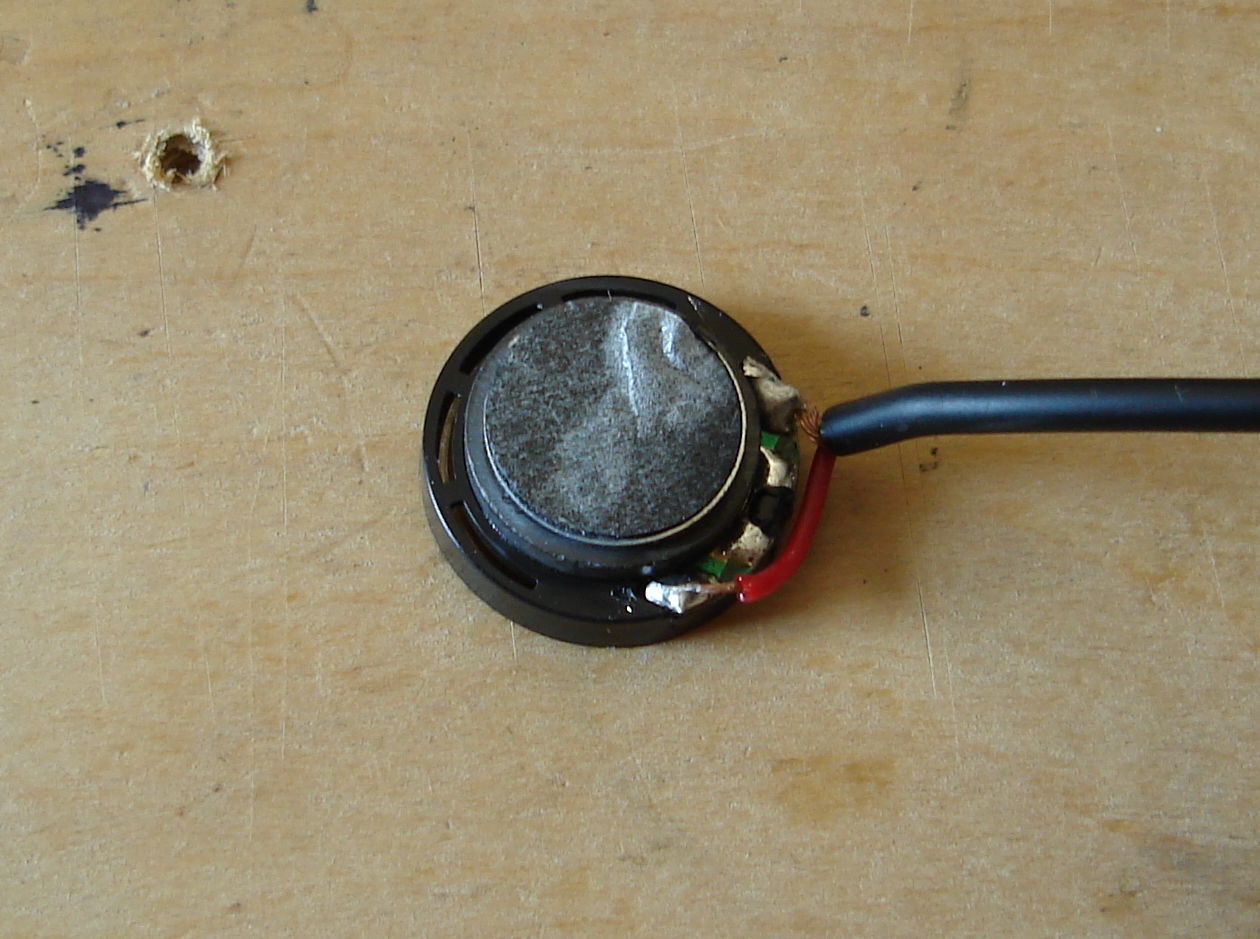
\includegraphics[width=6cm]{speaker_back.jpg}
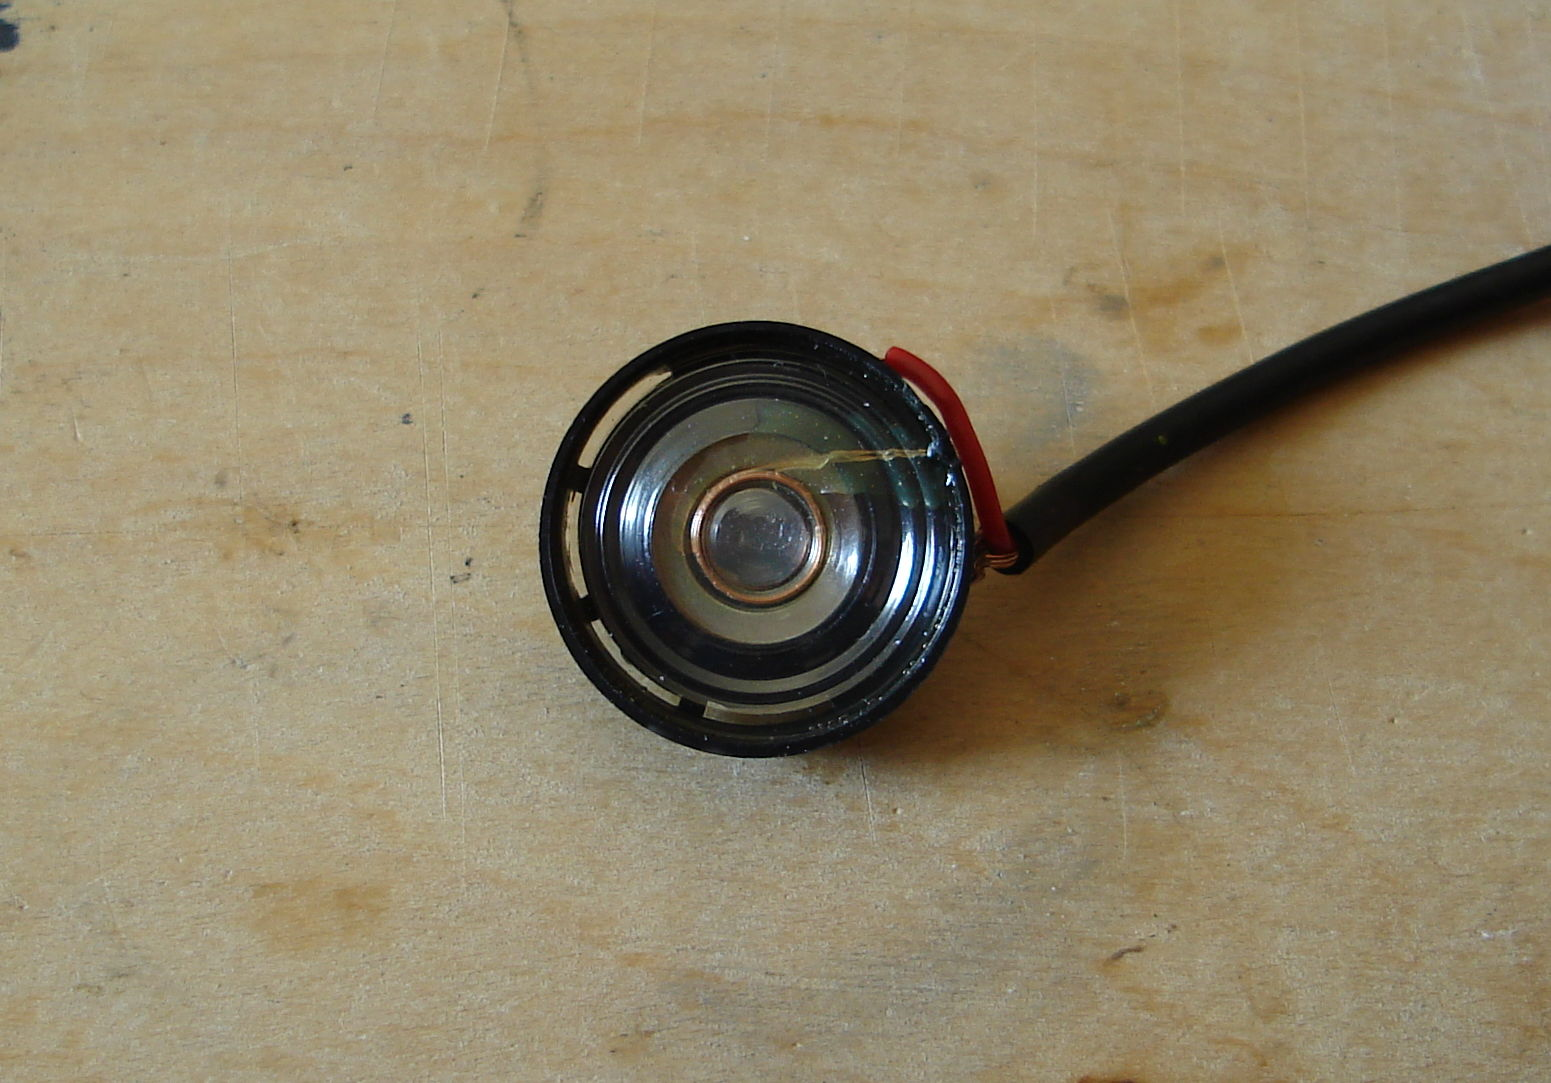
\includegraphics[width=6cm]{speaker_front.jpg}
\end{center}
\caption{Den separerede h�jttaler med lodninger.}
\label{lodning}
\end{figure}


Vores close-range m�linger er alle lavet ved 12 cm afstand, hhv. med og
uden kabinet, som det ses p� billederne i figur \ref{maalinger}.

Desuden har vi foretaget m�linger p� 2 m. afstand i en vinkel p�
ca. 45 grader oppe fra. Der er her lavet m�linger hvor h�jtaleren
peger hen imod lytteren, og v�k fra lytteren, for at afspejle hvad man
kan kalde almindeligt brug.

Alle m�lingerne er foretaget i et lydd�dt rum (se figur \ref{room}),
med en udefra d�mpning p� -60dB. Rummet er approksimativt $60m^3$ med
en nedre begr�nsende frekvens p� 100Hz, svarende til starten p� vores
sweep (100Hz - 20kHz).

\begin{figure}[h!]
\begin{center}
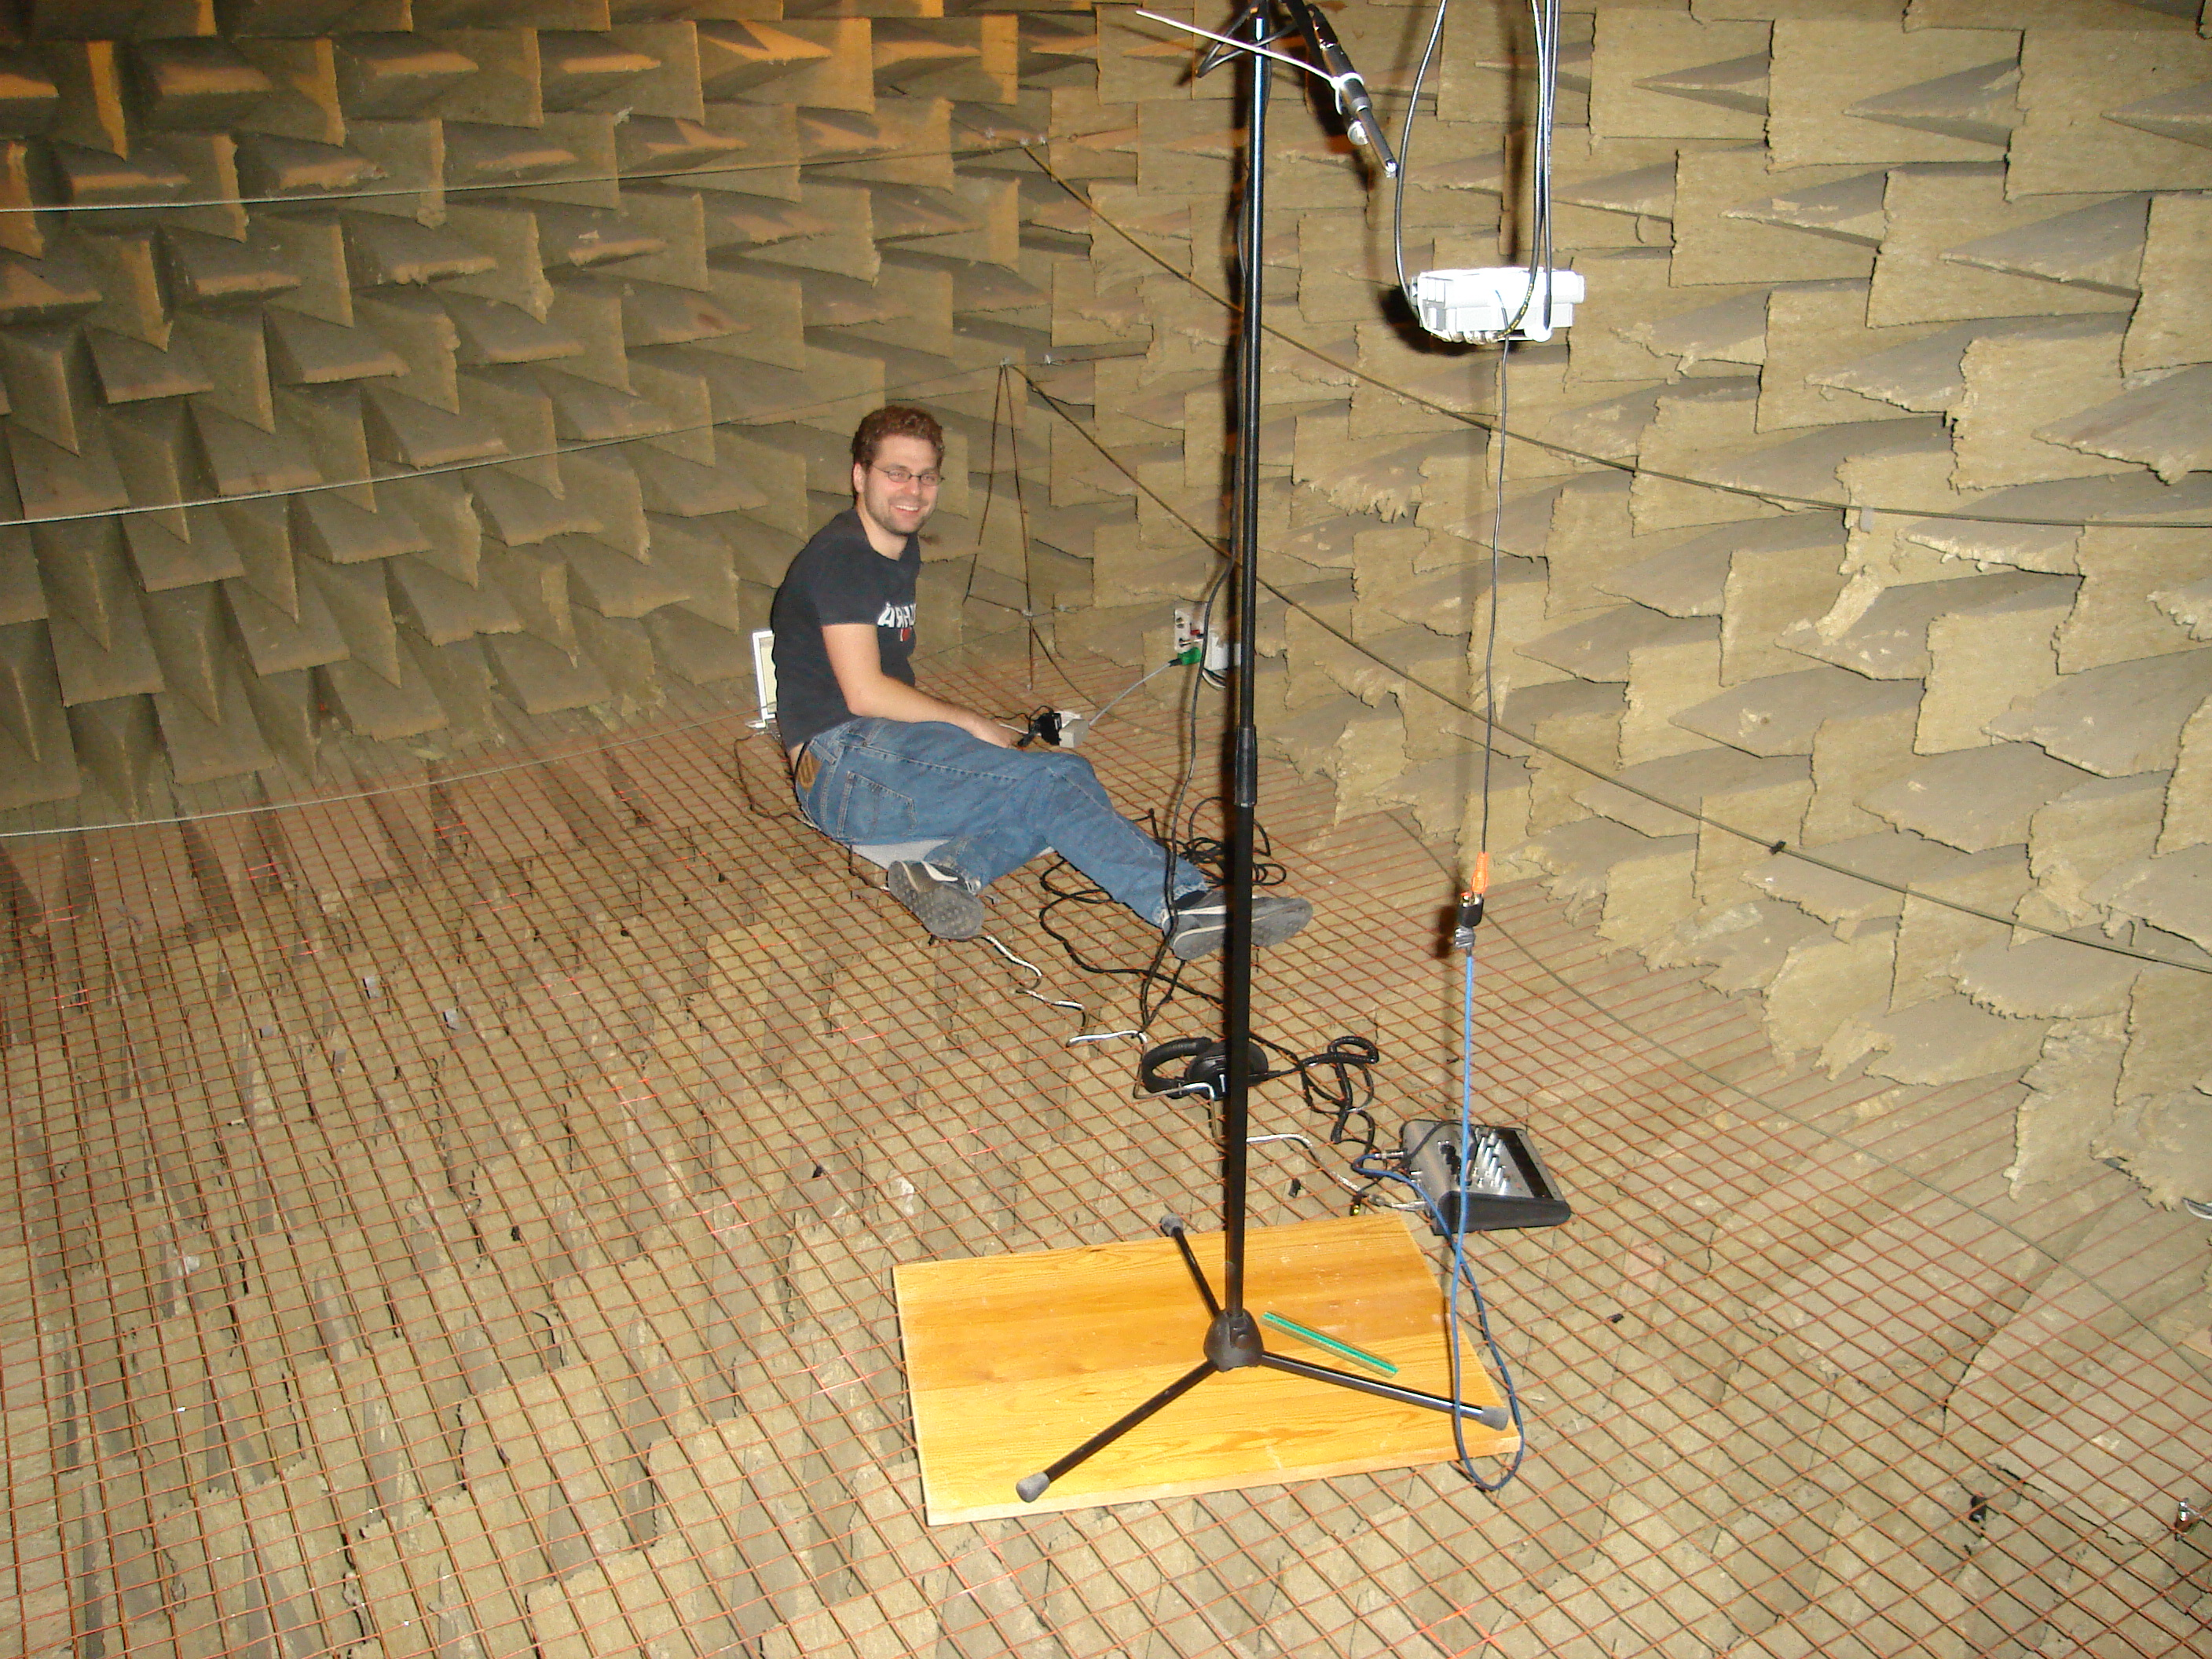
\includegraphics[width=12cm]{room.jpg}
\end{center}
\caption{M�linger blev foretaget i et lydd�dt rum.}
\label{room}
\end{figure}

\begin{figure}[h!]
\begin{center}
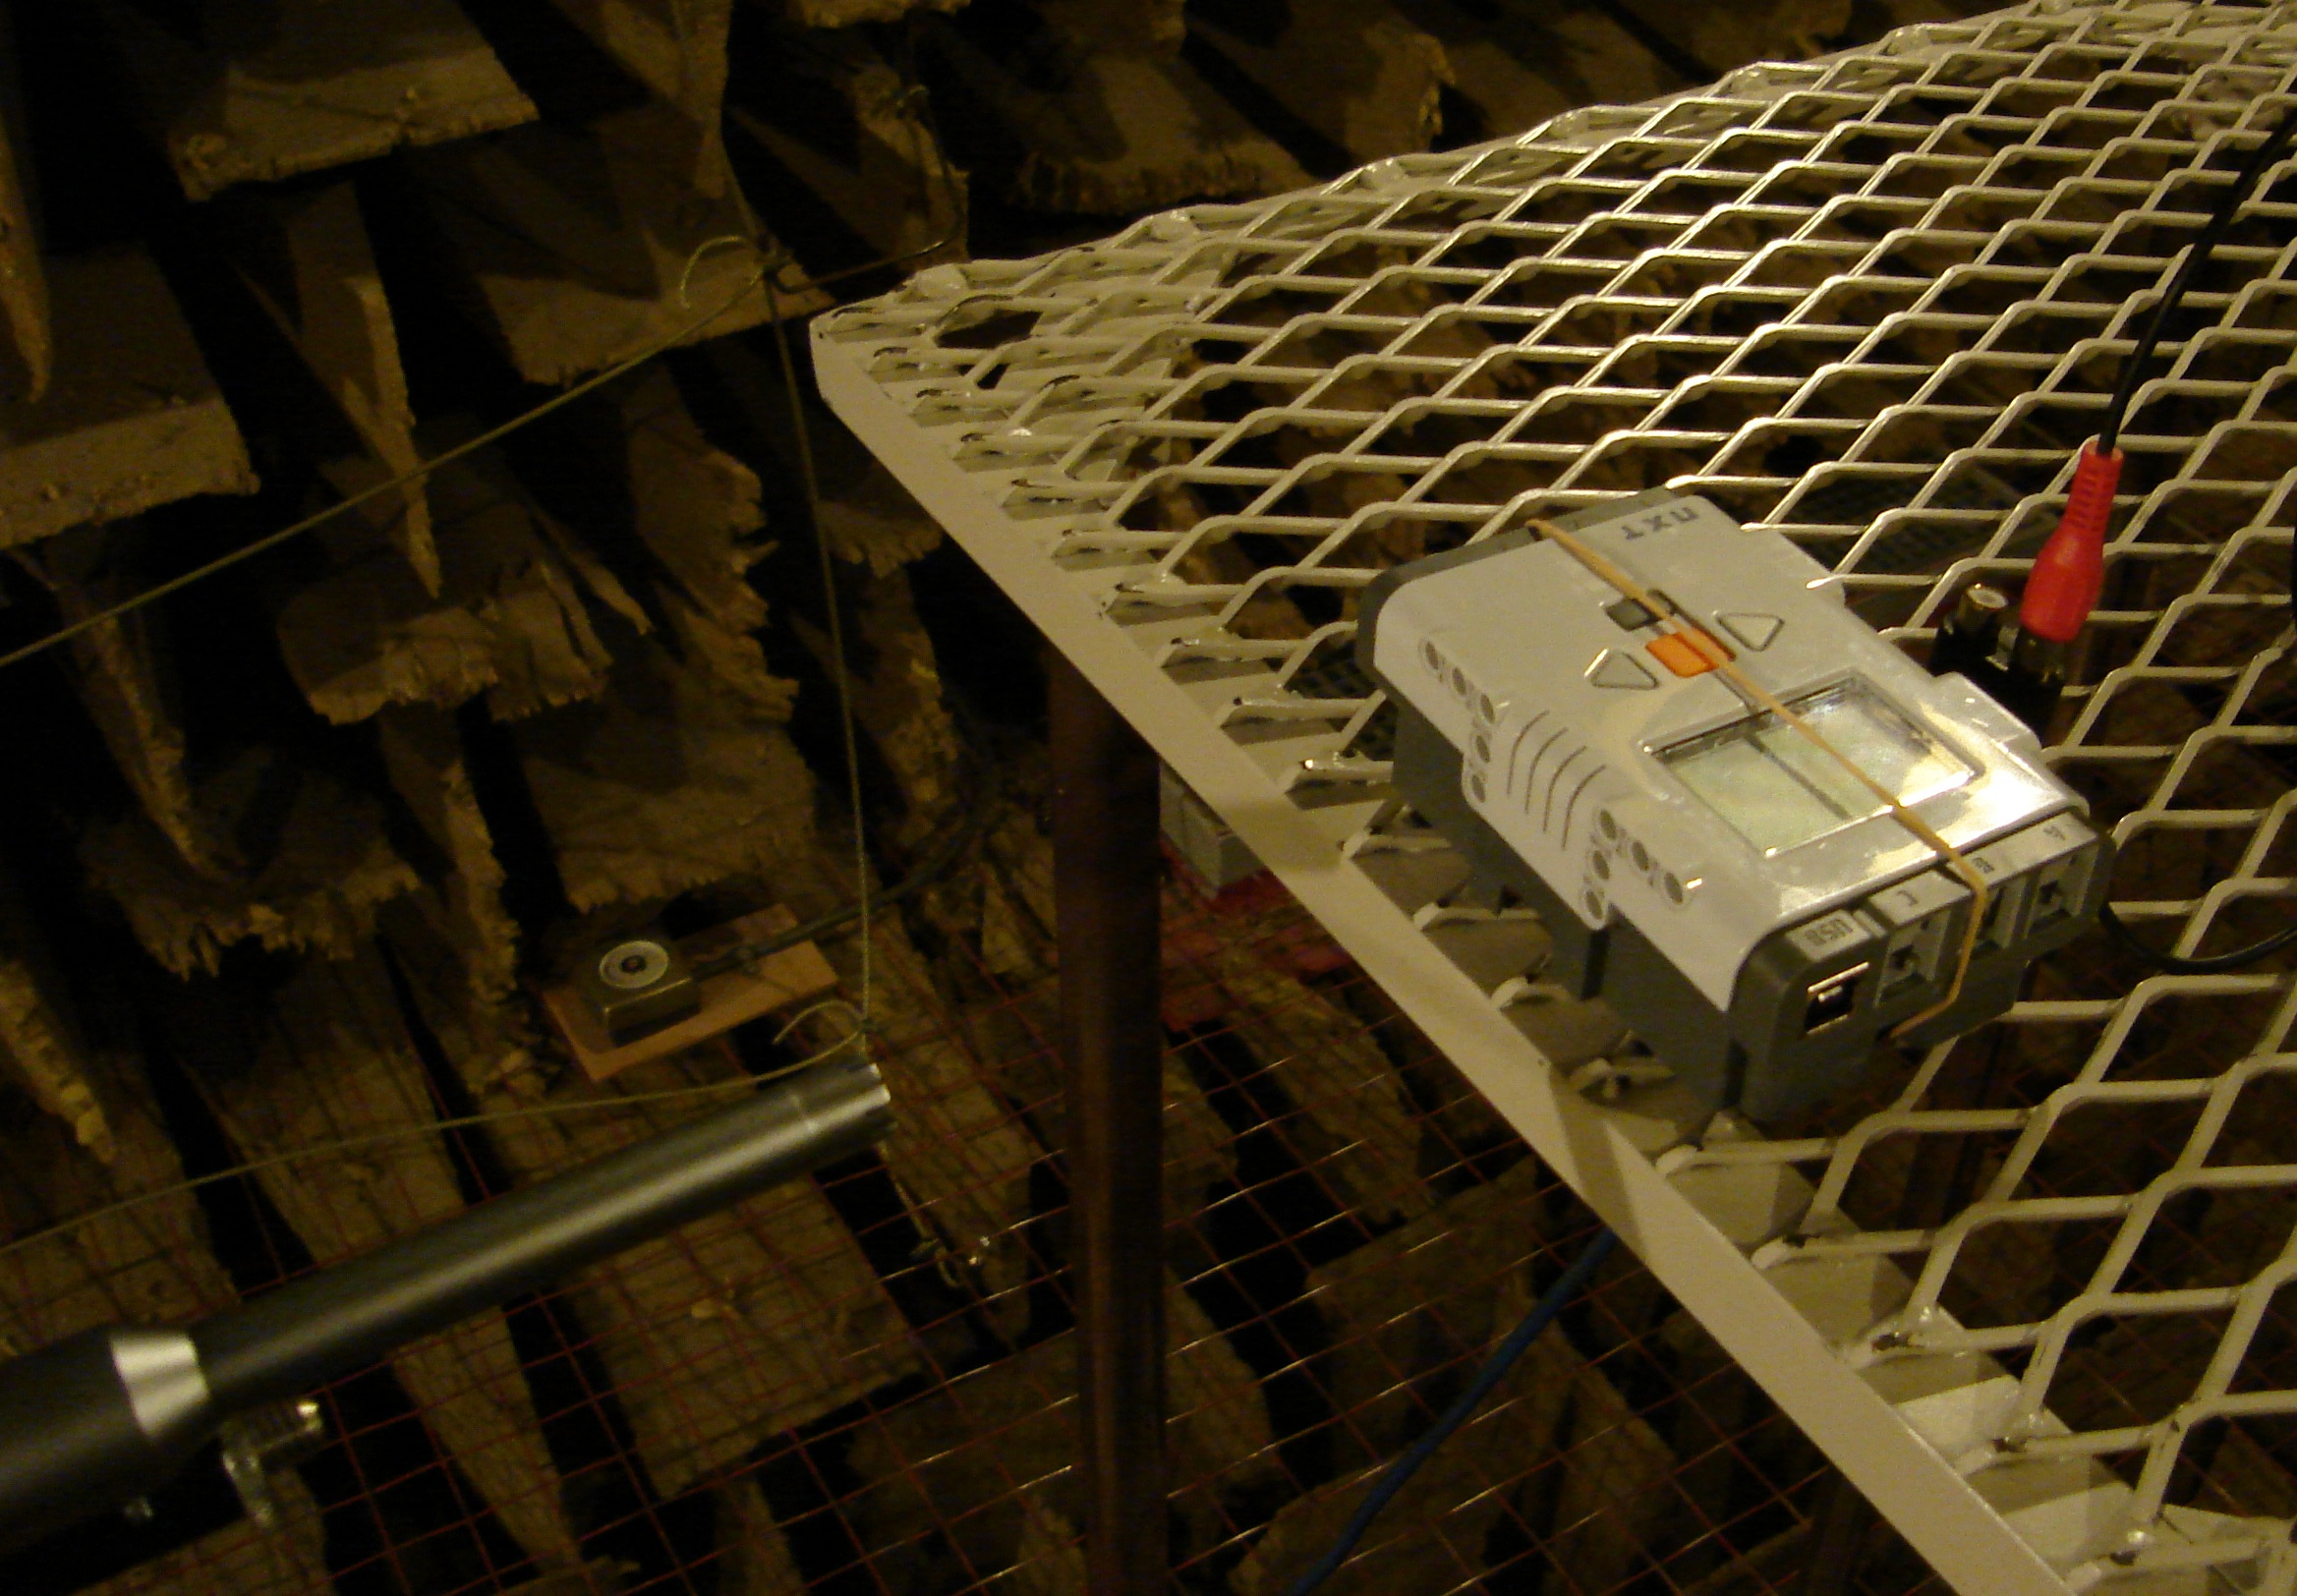
\includegraphics[width=6cm]{maaling_kabinet.jpg}
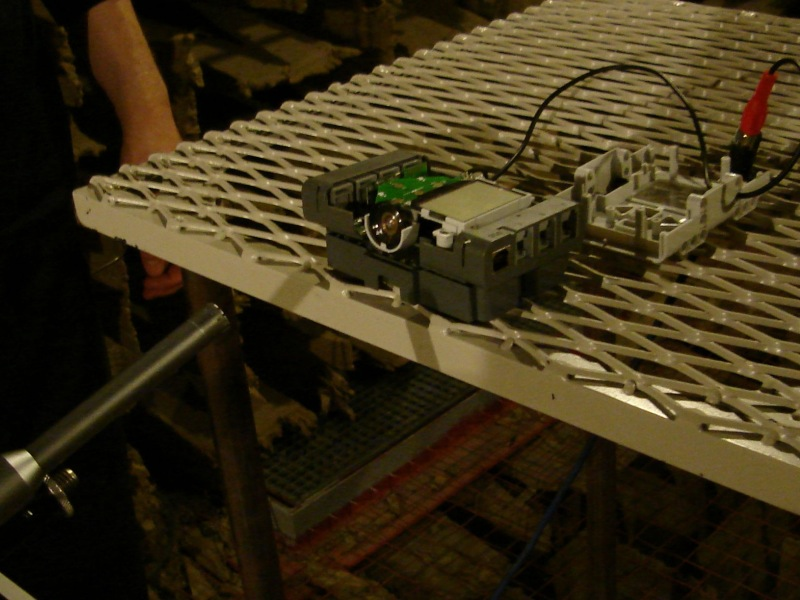
\includegraphics[width=6cm]{maaling_nokabinet.jpg}
\end{center}
\caption{M�lingerne blev foretaget b�de med og uden kabinet i 12cm afstand.}
\label{maalinger}
\end{figure}

\section{Resultater}
% impulsrespons
\begin{figure}[h!]
\begin{center}
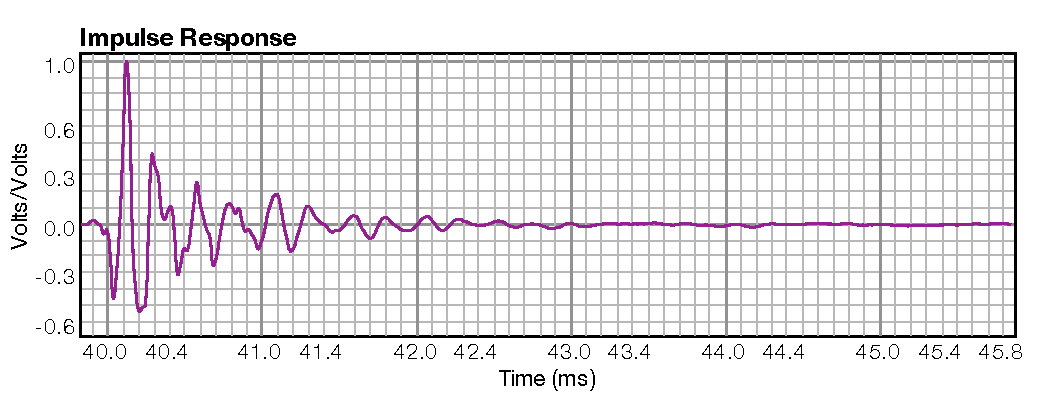
\includegraphics[width=12cm]{impulsrespons.pdf}
\end{center}
\caption{H�jttalerens impulsrespons, on-axis med kabinet}
\label{impuls}
\end{figure}
%
% alle paa een gang, shell, no+shell
\begin{figure}
\begin{center}
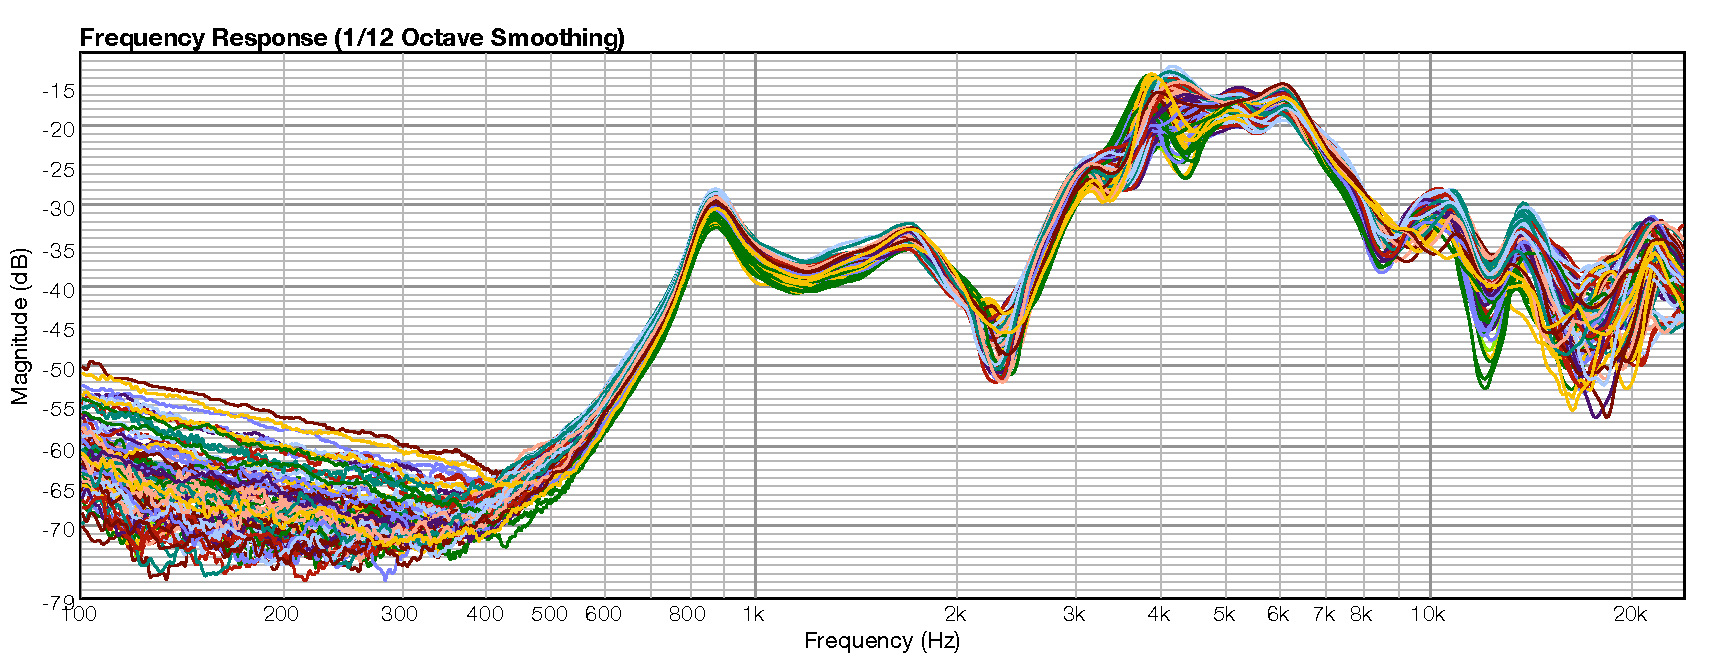
\includegraphics[height=6cm,angle=-90]{shell-all.pdf}
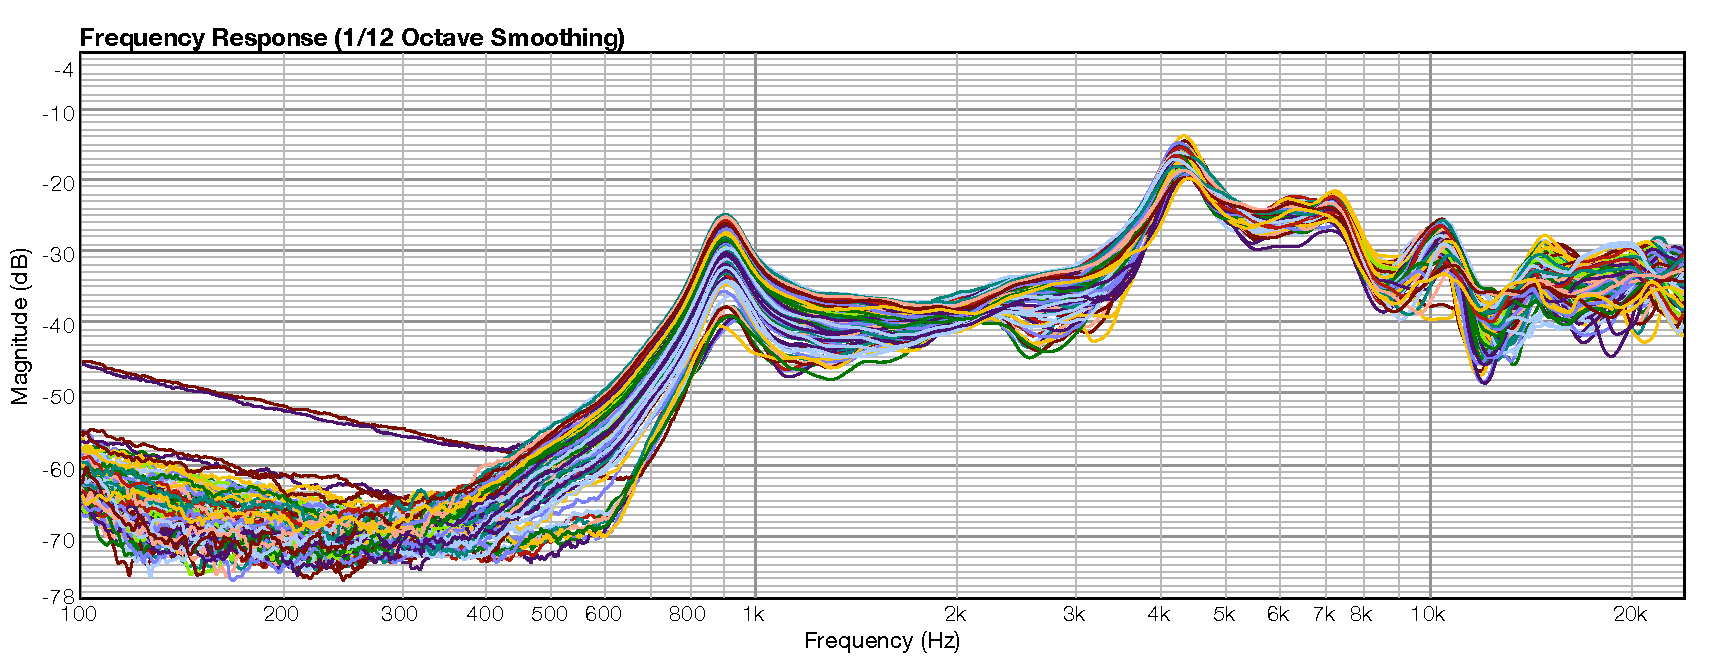
\includegraphics[height=6cm,angle=-90]{noshell-all.pdf}
\end{center}
\caption{Alle m�linger, venstre med kabinet, h�jre uden kabinet}
\label{all}
\end{figure}
%
% on-axis med og uden kabinet
\begin{figure}
\begin{center}
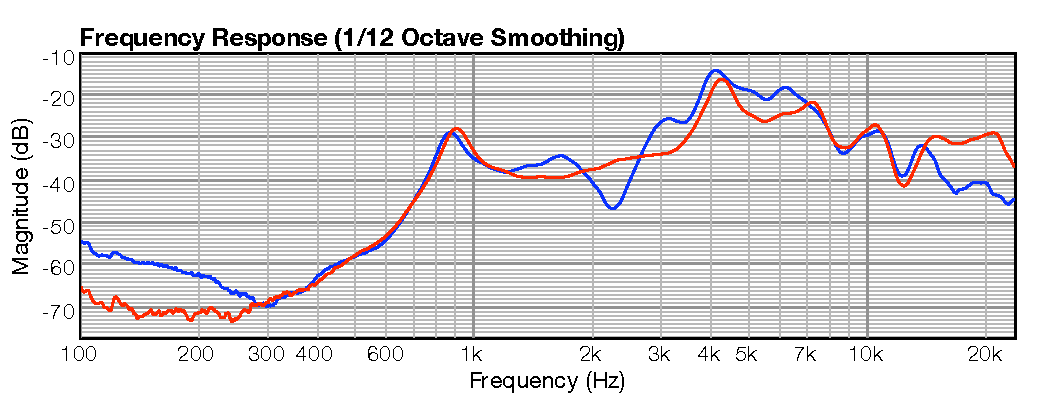
\includegraphics[height=6cm,angle=-90]{onaxis-shell-noshell.pdf}
\end{center}
\caption{On-axis, bl�: med kabinet, r�d: uden kabinet}
\label{onaxis}
\end{figure}
%
% on-axis med kabinet og s� -40 til 0 horisontalt
% on-axis med kabinet og s� -40 til 0 vertikalt
\begin{figure}
\begin{center}
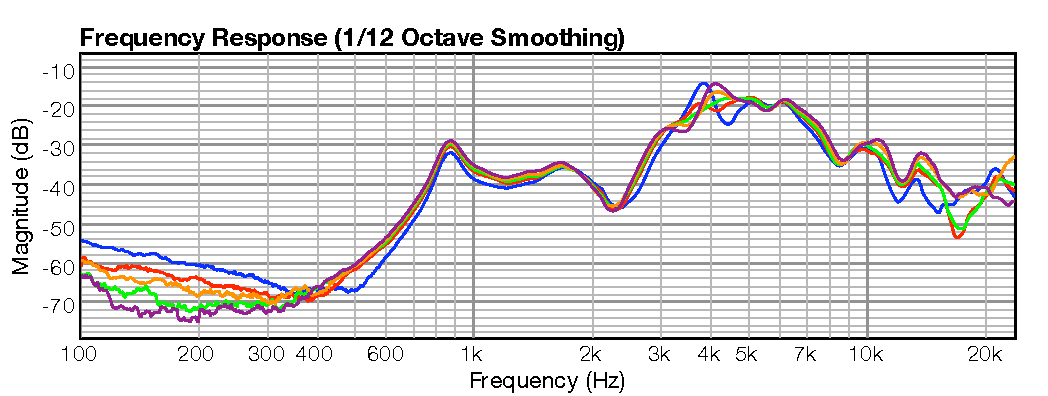
\includegraphics[height=6cm,angle=-90]{minus40to0horizontal.pdf}
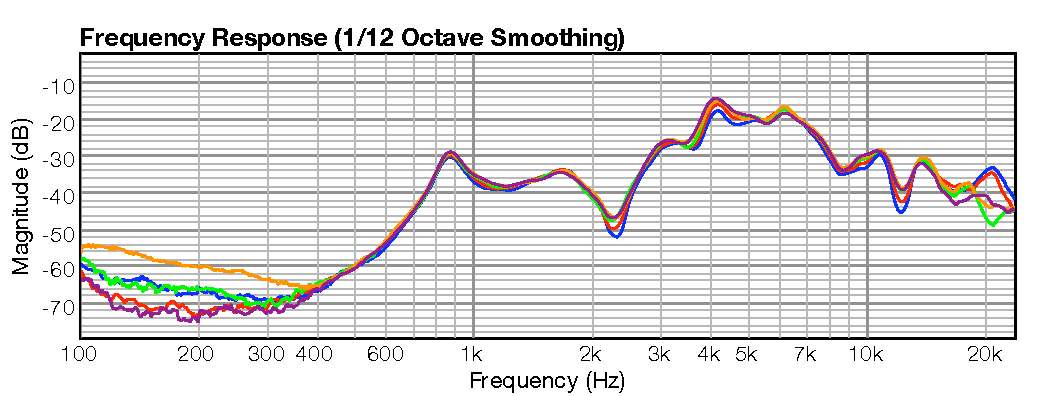
\includegraphics[height=6cm,angle=-90]{minus40to0vertical.pdf}
\end{center}
\caption{M�linger med vinkel-sweep, venstre horisontalt, h�jre
  vertikalt. Bl�: $-40\,^{\circ}$ , r�d: $-30\,^{\circ}$, gr�n:
  $-20\,^{\circ}$, orange: $-10\,^{\circ}$, lilla: $0\,^{\circ}$ (on-axis)}
\label{orto}
\end{figure}
%
% to meter v�k, b�de hen mod lytteren og v�k fra lytteren
\begin{figure}
\begin{center}
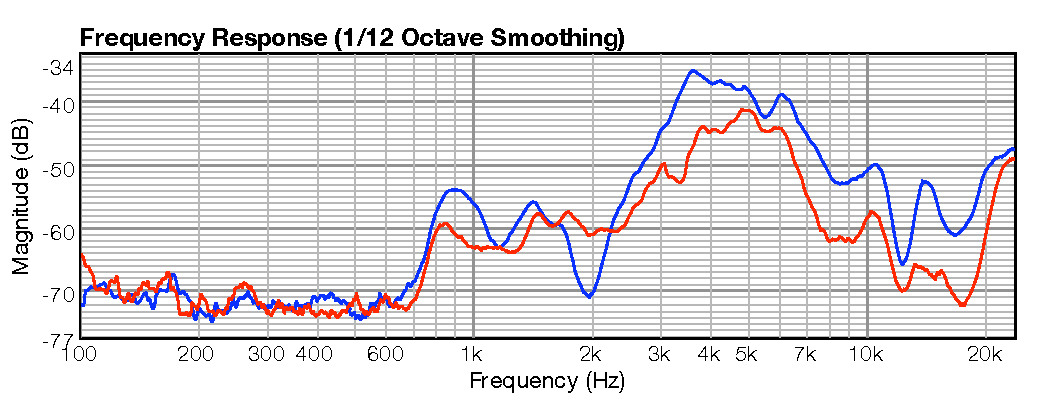
\includegraphics[height=6cm,angle=-90]{2mdist.pdf}
\end{center}
\caption{2 meters afstand, bl�: imod mikrofonen, r�d: v�k fra mikrofonen}
\label{2mdist}
\end{figure}

\section{Analyse}
\subsection*{H�jttalerens impulsrespons}
Af figur \ref{impuls} ses, at impulsresponset er forholdsvist kort, ca. 5 ms, hvilket natuligvis stemmer overens med, at responset er optaget i et lydd�dt rum.

\subsection*{Frekvenskarakteristikken generelt}
I figur \ref{all} er alle m�lingerne vist samlet med og uden NXT-kabinettet p�sat. Generelt fremg�r det, at h�jttaleren ikke siger meget under 600 Hz, hvilket naturligvis h�nger sammen med h�jttalerens diameter p� ca. 30 mm. Derudover observeres en line�r frekvensgang set i forhold til at det er en lille h�jttaler.

\subsection*{Spredningskarakteristik og kabinettets p�virkning}
I figur \ref{orto}, sammenholdes m�linger med vinkler mellem $-40\,^{\circ}$ og $0\,^{\circ}$ horisontalt og vertikalt. Dette illustrerer h�jttalerens spredningskarakteristik, og det fremg�r at vinklen ikke betyder det store for frekvensspektret.

Der er dog generelt st�rre spredning p� m�lingerne ved den horisontale vinkel�ndring, hvilket kan skyldes p�virkning fra kabinettets vertikale riller, se figur \ref{kabinet}.

\begin{figure}[h!]
\begin{center}
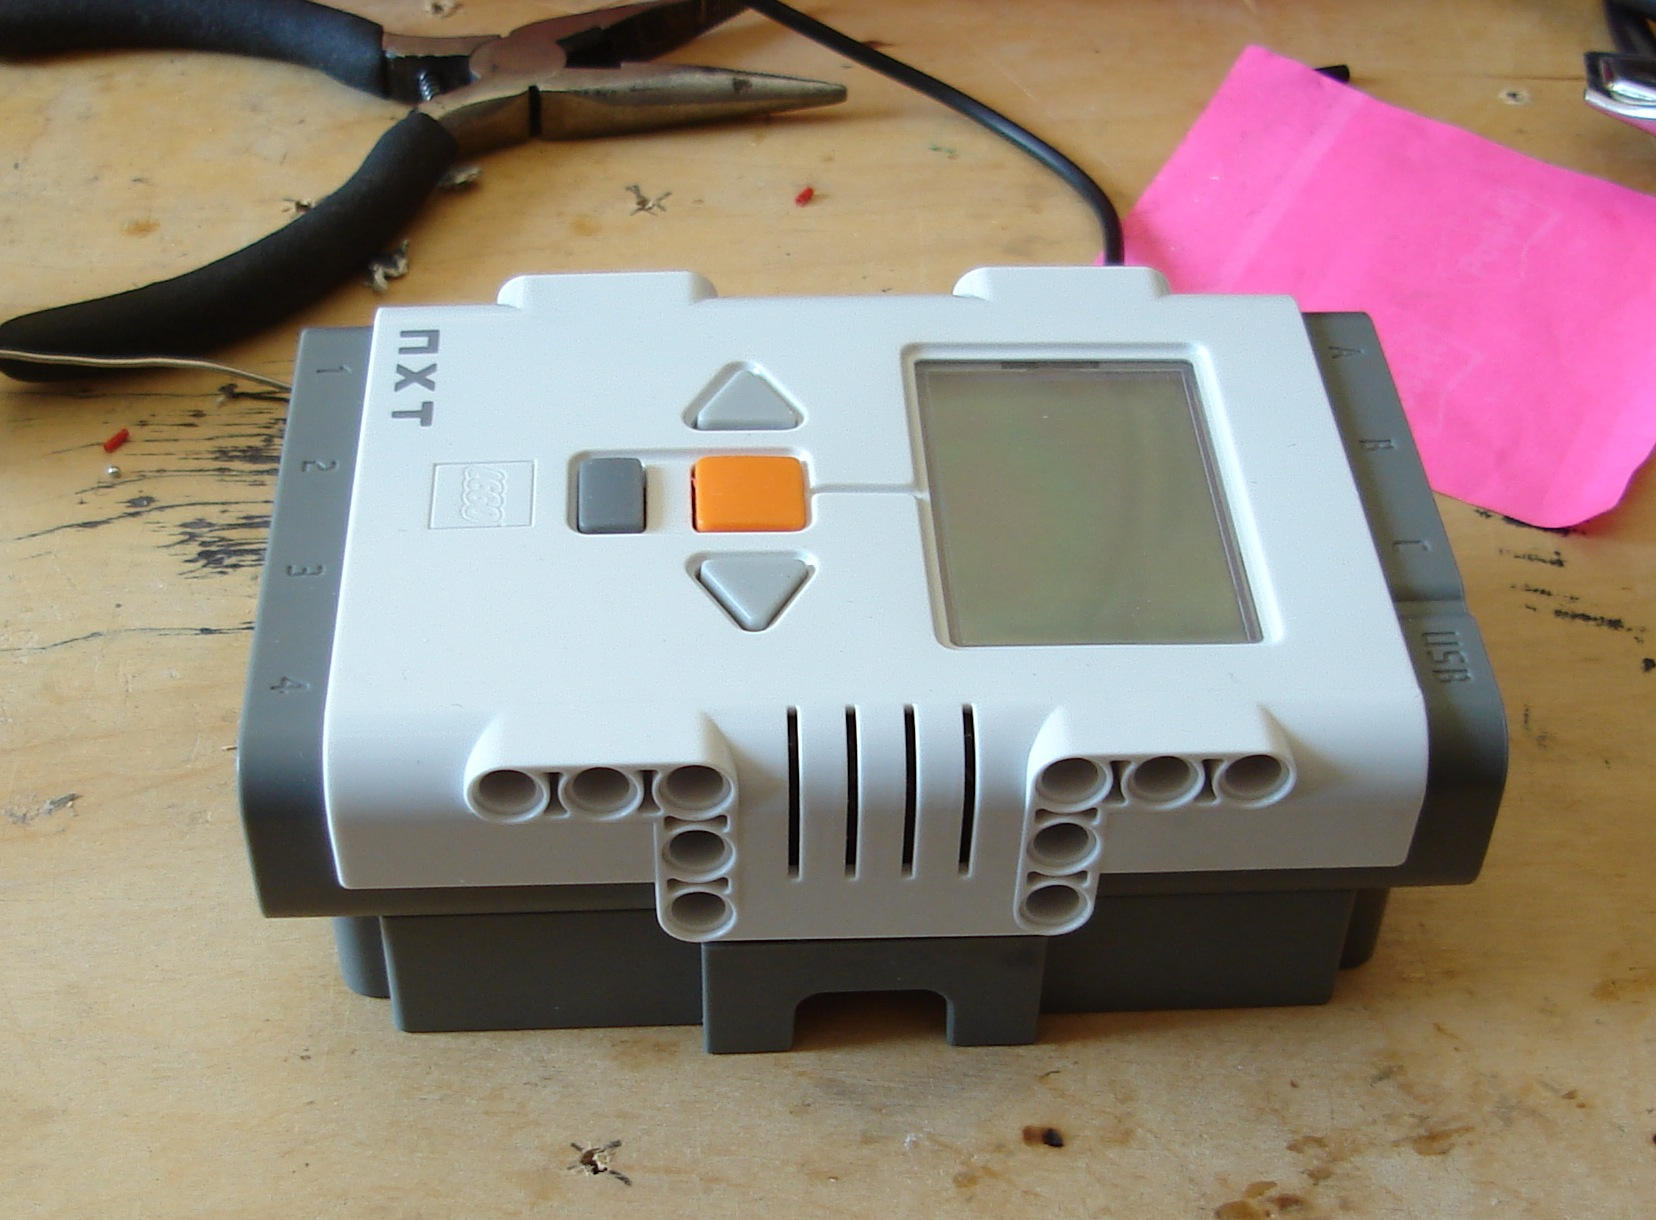
\includegraphics[width=8cm]{kabinet.jpg}
\end{center}
\caption{NXT'ens kabinet med de vertikale riller}
\label{kabinet}
\end{figure}

I figur \ref{onaxis} sammenlignes on-axis m�linger for h�jttaleren med og uden NXT-kabinettet p�sat. Det ses at kabinettet giver en betydelig p�virkning ved godt 2 kHz med et dyk p� ca. 10 dB. 


\section{Evaluering}
Sammenhold med Peters resultater

Mikkel:
Gang vores frekvensrespons sammen med Peters

Som det fremg�r af frekvensresponset giver NXT'ens kredsl�b et high-cut allerede ved omkring 1 kHz, mens h�jttaleren f�rst begynder at respondere ved 600 Hz. Dette efterlader et meget begr�nset frekvensspekter something something.


generelt, hvad egner h�jttaleren sig til (musik/bip-lyde/taler)
Egner h�jttaleren sig til det den er t�nkt til?

Forslag til korrigering osv





Vi har i denne �velse lavet en succesfuld implementation af den kvantisering, som benyttes i JPEG. Vi har ogs� implementeret Huffman-encoding, prim�rt for at estimere komprimeringsfaktoren, men vores encoding kan ogs� udvides til at gemme billedet p� disken og senere decode det.

Vi har i vores program givet mulighed for at eksperimentere med kvantiseringen og f� vist resultatet, b�de grafisk samt i form af en PSNR v�rdi.


%\includeonly{filename,filename,...}

%Denne opgave er skrevet ved brug af \LaTeX2e
\end{document}
%*********************************************
%*                 end of                    *
%*              -=DOCUMENT=-                 *
%*********************************************
